\chapter{Introduction to Raman spectroscopy}
\label{ch:introduction}

The Raman effect was first reported by the physicist Chandrasekhara Venkata Raman in 1928 and later recognized with the Nobel Prize in Physics in 1930. When light interacts with matter, a small fraction of the incident radiation can exchange energy with the vibrational modes of the molecules in the sample, producing frequency shifts in the scattered light.

Raman spectroscopy is a vibrational spectroscopic technique used to investigate the molecular composition and structure of a sample through its interaction with light, by measuring these shifts. Since vibrational frequencies depend on chemical bonds, molecular masses and local structure, the resulting spectral pattern carries chemically specific information. A Raman spectrum can therefore be interpreted as a vibrational fingerprint of the material under investigation.

\section{Physical description of the Raman effect}
\label{sec:theory_raman_effect}

\subsection{Classical theory: induced dipole and polarizability}
\label{subsec:classical_raman}

The Raman effect can be introduced by following the response of a molecule to the electric field of the incident radiation. In a classical description, the molecule is treated as a polarizable object: the external field slightly displaces the electronic cloud with respect to the nuclei, and this displacement creates an induced electric dipole. The electric field of a monochromatic laser beam can be written as
\begin{equation}
    \mathbf{E}(t) = \mathbf{E}_0 \cos(2\pi \nu_0 t),
    \label{eq:incident_field}
\end{equation}
where \(\mathbf{E}_0\) is the field amplitude and \(\nu_0\) is the frequency of the exciting radiation. To first order, the induced dipole is proportional to the applied field:
\begin{equation}
    \boldsymbol{\mu}_{\mathrm{ind}}(t) =
    \boldsymbol{\alpha}\mathbf{E}(t),
    \label{eq:induced_dipole}
\end{equation}
where \(\boldsymbol{\alpha}\) is the polarizability tensor. Polarizability measures how easily the electronic distribution can be deformed by an external electric field. In this view, scattering is the radiation emitted by the induced dipole as it oscillates under the action of the incident wave.

\subsection{Molecular vibrations and Raman activity}
\label{subsec:molecular_vibrations}

If the molecule were fixed at its equilibrium geometry, the polarizability would be constant and the induced dipole would oscillate only at the laser frequency. The emitted radiation would therefore have the same frequency as the incident radiation, producing an elastic process known as Rayleigh scattering. Raman scattering appears when nuclear motion is taken into account.

The effect of nuclear motion on polarizability can be explained by recalling the mechanical picture behind molecular vibrations. A chemical bond has an equilibrium geometry, corresponding to the minimum of its potential energy curve. A real bond is more accurately described by an anharmonic Morse-like potential; however, for small displacements around equilibrium, this potential can be approximated by a parabola. In this harmonic approximation, the restoring force is proportional to the displacement, according to Hooke's law, and the bond can be treated as an elastic connection.
In the simplest diatomic case, the molecule behaves like two masses connected by a spring, and the vibrational frequency depends on both the stiffness of the bond and the reduced mass of the two atoms. Stiffer bonds lead to higher vibrational frequencies, while heavier atoms generally lead to lower ones. In a polyatomic molecule, the nuclear motion is more complex, but it can be decomposed into independent collective motions called normal modes. Each normal mode is described by a coordinate \(Q_k\), which represents a coordinated displacement pattern of the nuclei rather than the motion of a single atom. This description is useful for Raman scattering because changes in the nuclear geometry can modify the electronic distribution, and therefore the polarizability, along each normal coordinate.

In the harmonic approximation, each normal coordinate oscillates sinusoidally around the equilibrium geometry:
\begin{equation}
    Q_k(t) = Q_{k,0}\cos(2\pi \nu_k t),
    \label{eq:normal_coordinate}
\end{equation}
where \(\nu_k\) is the vibrational frequency of the \(k\)-th normal mode.

\begin{figure}[htbp]
    \centering
    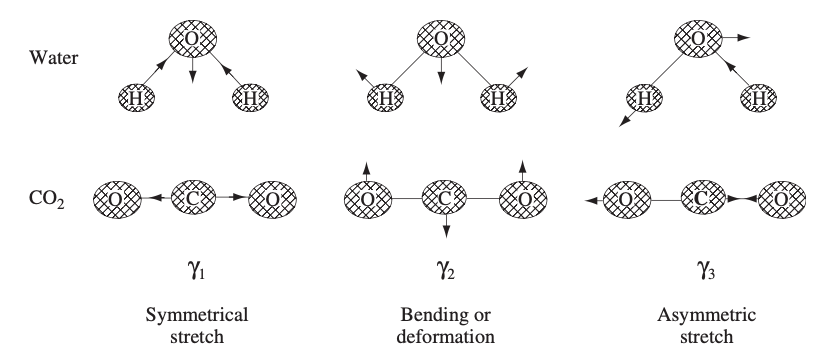
\includegraphics[width=0.70\textwidth]{Images/images_ch_1/normal_modes.png}
    \caption{Examples of normal vibrational modes in simple molecules. Each mode corresponds to a coordinated displacement pattern of the nuclei, such as symmetric stretching, bending or asymmetric stretching \cite{smith2005modernraman}.}
    \label{fig:normal_modes}
\end{figure}

During this motion, the molecular geometry changes, and the polarizability may change accordingly. Expanding a component of the polarizability tensor around the equilibrium configuration gives
\begin{equation}
    \alpha_{ij}(\{Q\}) \simeq
    \left(\alpha_{ij}\right)_0 +
    \sum_k
    \left(\frac{\partial \alpha_{ij}}{\partial Q_k}\right)_0 Q_k  
    \label{eq:polarizability_taylor}
\end{equation}
The constant term in equation~\eqref{eq:polarizability_taylor} describes the polarizability of the molecule at equilibrium; the linear term describes how that polarizability changes when the nuclei move along a vibrational coordinate. Substituting equations~\eqref{eq:incident_field} and \eqref{eq:normal_coordinate} into equation~\eqref{eq:induced_dipole}, and retaining the first-order term of equation~\eqref{eq:polarizability_taylor}, gives
\begin{equation}
\begin{aligned}
    \mu_{\mathrm{ind}}(t) \propto {}&
    \underbrace{\alpha_0 E_0 \cos(2\pi \nu_0 t)}_{\text{Rayleigh}} \\
    &+
    \underbrace{\frac{1}{2}
    \left(\frac{\partial \alpha}{\partial Q_k}\right)_0
    Q_{k,0}E_0
    \cos 2\pi(\nu_0-\nu_k)t}_{\text{Stokes}} \\
    &+
    \underbrace{\frac{1}{2}
    \left(\frac{\partial \alpha}{\partial Q_k}\right)_0
    Q_{k,0}E_0
    \cos 2\pi(\nu_0+\nu_k)t}_{\text{anti-Stokes}} .
\end{aligned}
\label{eq:induced_dipole_components}
\end{equation}
This expression contains the essential result of the classical treatment. The first term, proportional to \(\alpha_0\), oscillates at the laser frequency \(\nu_0\) and corresponds to Rayleigh scattering.  The other terms arise only if the vibration changes the polarizability. They oscillate at \(\nu_0-\nu_k\) and \(\nu_0+\nu_k\), which correspond to the Stokes and anti-Stokes Raman components, respectively. In this sense, Raman scattering can be understood as a frequency modulation of the induced dipole caused by molecular vibration.

A vibrational mode contributes to the Raman spectrum only if it changes at least one component of the polarizability tensor:
\begin{equation}
    \left(\frac{\partial \alpha_{ij}}{\partial Q_k}\right)_0 \neq 0.
    \label{eq:raman_activity}
\end{equation}
In physical terms, this means that the vibration must modify the response of the electronic cloud to the incident electric field, by changing the ease with which the cloud can be distorted.

\subsection{Quantum interpretation: vibrational levels and virtual states}
\label{subsec:quantum_raman}

The classical description explains the origin of the shifted frequencies, but it does not account for the quantization of molecular vibrational energy or for the different populations of the initial vibrational states. A quantum interpretation is therefore needed to describe Raman scattering in terms of transitions between vibrational levels.
 
 In a quantum picture, the vibrational energy of the molecule is quantized, and the molecule occupies discrete vibrational states, denoted by quantum numbers \(\nu = 0, 1, 2, \ldots\).
 
 \begin{figure}[htbp]
    \centering
    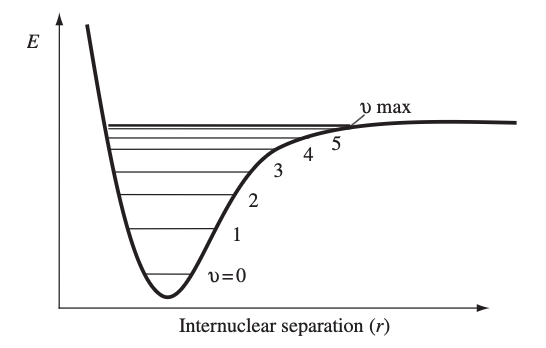
\includegraphics[width=0.55\textwidth]{Images/images_ch_1/molecular_vibrational_states.png}
    \caption{A typical Morse curve for an electronic state showing the vibrational levels as horizontal tie lines \cite{smith2005modernraman}.}
    \label{fig:molecular_vibrational_states}
\end{figure}
 
  When radiation interacts with the molecule the oscillating electric field distorts the electronic cloud and forms a very short-lived  complex, usually described as a virtual state. This state is not a stable eigenstate of the isolated molecule and exists only during the scattering event. The system then relaxes almost immediately by emitting a scattered photon.

In Rayleigh scattering, the molecule returns to the same vibrational state from which it started, and the scattered photon has the same energy as the incident photon. In Stokes Raman scattering, the molecule ends in a higher vibrational state; part of the incident photon energy remains in the molecule, so the scattered photon has lower energy compared to the incident photon. In anti-Stokes Raman scattering, the molecule is initially in an excited vibrational state and returns to a lower one; vibrational energy is transferred from the molecule to the photon, so the scattered photon has higher energy.

\begin{figure}[htbp]
    \centering
    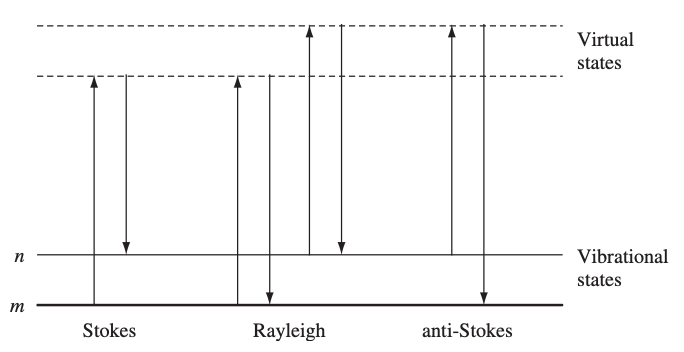
\includegraphics[width=0.65\textwidth]{Images/images_ch_1/stokes_and_anti_stokes.png}
    \caption{Energy-level representation of Rayleigh, Stokes and anti-Stokes scattering \cite{smith2005modernraman}.}
    \label{fig:stokes_anti_stokes}
\end{figure}

\subsection{Selection rules}
\label{subsec:selection_rules}

The probability of such a transition is not determined simply by the existence of two energy levels, but by how strongly the two states are coupled by the molecular response to the field. This is why the quantum description naturally introduces matrix elements: they express whether a transition between two vibrational states is allowed and how efficiently it can occur. The probability of a Raman transition between an initial vibrational state \(|i\rangle\) and a final state \(|f\rangle\) is proportional to the squared modulus of the polarizability matrix element:
\begin{equation}
    P_{i\rightarrow f}^{\mathrm{Raman}} \propto
    \left|\alpha_{fi}\right|^2,
    \qquad
    \alpha_{fi} = \langle f|\hat{\alpha}|i\rangle .
    \label{eq:raman_transition_probability}
\end{equation}
Using the first-order expansion of polarizability, the probability amplitude for the Raman transition contains a term that couples the initial and final vibrational states through the coordinate \(Q_k\):
\begin{equation}
    \alpha_{fi}^{\mathrm{Raman}} \propto
    \left(\frac{\partial \alpha}{\partial Q_k}\right)_0
    \langle v_f|Q_k|v_i\rangle .
    \label{eq:raman_matrix_element}
\end{equation}
This equation links the classical and quantum descriptions. The derivative of the polarizability gives the Raman activity condition, while the matrix element of \(Q_k\) gives the vibrational selection rule for the mode considered. In a molecule with several normal modes, the same idea can be written more explicitly as
\begin{equation}
    \alpha_{fi}^{\mathrm{Raman}} \propto
    \sum_k
    \left(\frac{\partial \alpha}{\partial Q_k}\right)_0
    \langle v_{f,k}|Q_k|v_{i,k}\rangle
    \prod_{j\neq k}
    \langle v_{f,j}|v_{i,j}\rangle .
    \label{eq:raman_matrix_element_multimode}
\end{equation}
The factor \(\langle v_{f,k}|Q_k|v_{i,k}\rangle\) describes the transition of the active mode \(k\). In the harmonic approximation, it is non-zero only for \(\Delta v_k=\pm 1\). The product over \(j\neq k\) contains overlap integrals for all the other modes. Since different harmonic oscillator states are orthogonal, these factors are non-zero only when the final and initial quantum numbers are the same for those modes. Therefore, in a fundamental Raman transition, one normal mode changes by one quantum, while the other normal modes remain unchanged. The Stokes process corresponds to \(\Delta v_k=+1\), while the anti-Stokes process corresponds to \(\Delta v_k=-1\).

The quantum picture also explains why Stokes lines are usually more intense than anti-Stokes lines. At thermal equilibrium, most molecules occupy the lowest vibrational state, while only a smaller fraction is already vibrationally excited. Stokes scattering can therefore start from the most populated state, whereas anti-Stokes scattering requires the molecule to be in an excited vibrational state before the interaction with the photon. As temperature increases, the population of excited vibrational states also increases, and the anti-Stokes signal can become stronger. Under ordinary experimental conditions, however, this population is usually small for many vibrational modes. This is why biological Raman measurements commonly focus on the Stokes side of the spectrum.

\subsection{Raman shift and spectral representation}
\label{subsec:raman_shifts}

In practice, Raman spectra are not usually represented as a function of the absolute wavelength of the scattered light. The horizontal axis is instead the Raman shift, defined as the difference between the wavenumber of the incident radiation and that of the scattered radiation. For Stokes scattering,
\begin{equation}
    \Delta \tilde{\nu} =
    \tilde{\nu}_0 - \tilde{\nu}_s =
    \frac{1}{\lambda_0} - \frac{1}{\lambda_s},
    \label{eq:raman_shift}
\end{equation}
and it is expressed in \(\mathrm{cm}^{-1}\). This representation is useful because Raman band positions correspond to vibrational energy differences and are therefore characteristic of the sample, independently of the excitation wavelength. In measured biological spectra, the intense Rayleigh component is removed by optical filters, so the useful spectrum is mainly composed of Raman bands, typically on the Stokes side.

\section{Raman spectroscopy for biological tissue characterization} 
\label{sec:raman_biological_tissues}

A Raman spectrum can be interpreted as a vibrational fingerprint of the sample. In simple molecules, individual bands may often be assigned to specific vibrational modes. In biological tissues, however, this fingerprint results from the superposition of many molecular contributions: tissues are chemically heterogeneous systems, and each measured spectrum combines signals from several molecular families, such as proteins, lipids, nucleic acids, carbohydrates, collagen and other extracellular matrix components. 

As a result, changes in tissue organization or biochemical composition do not usually affect a single isolated peak. Instead, they can modify relative intensities, band shapes, peak positions and correlations among different spectral regions. The information relevant for tissue characterization is distributed across the whole spectrum.

One spectral interval of particular interest is the \textbf{fingerprint region}, approximately between \(500\) and \(1800~\mathrm{cm}^{-1}\). This is generally the most chemically specific part of a biological Raman spectrum, since it contains bands associated with different molecular vibrations, including contributions from proteins, lipids, nucleic acids, carbohydrates and other tissue constituents. The overall pattern of peaks in this region can provide detailed information on the biochemical composition of the sample.

A second relevant interval is the \textbf{CH region}, around \(2800\)--\(3000~\mathrm{cm}^{-1}\), where C--H stretching vibrations are often observed. These bonds are abundant in biological molecules rich in carbon and hydrogen, especially lipids and proteins, making the signal from this region useful for tissue discrimination. However, its bands are usually broader and more overlapping than those in the fingerprint region, which makes individual molecular assignments less specific. Even so, their combined pattern can still carry class-relevant information.

The interval between the fingerprint and CH regions, approximately \(1800\)--\(2800~\mathrm{cm}^{-1}\), is often called the \textbf{silent region} because biological samples usually show few Raman bands in this range.

\begin{figure}[ht]
    \centering
    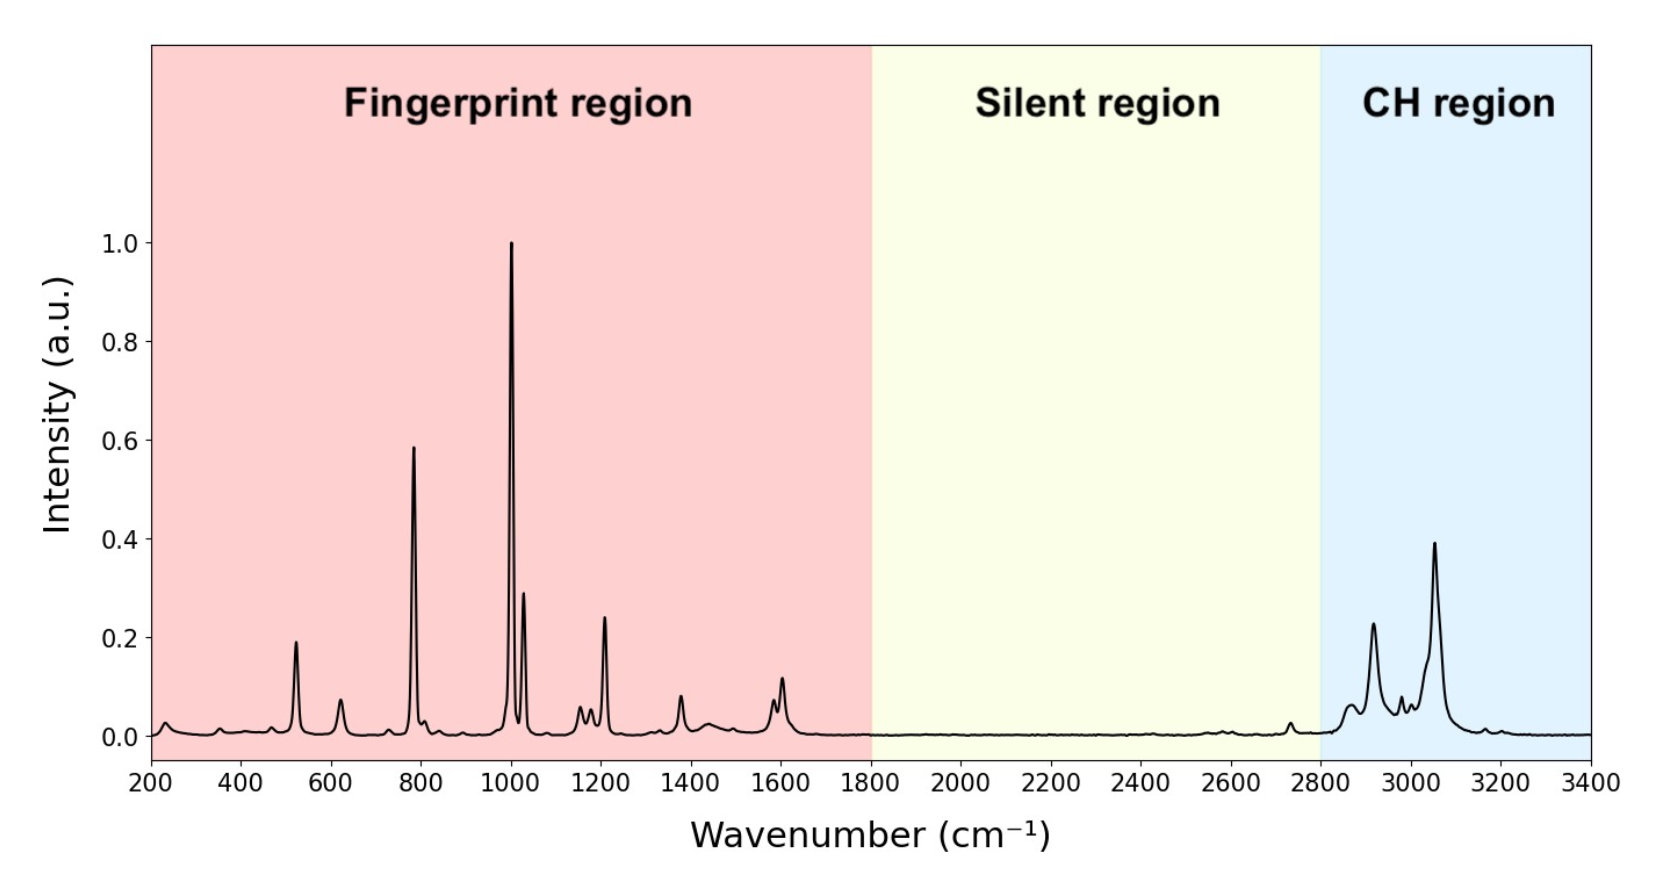
\includegraphics[width=0.65\textwidth]{Images/images_ch_1/regions.png}
    \caption{Representative Raman spectrum highlighting the main spectral regions considered in biological samples \cite{agrimi2025raman}.}
    \label{fig:raman_spectral_regions}
\end{figure}

For biological and clinical applications, Raman spectroscopy is relevant because it combines
chemical specificity with several practical advantages:
\begin{itemize}
    \item \textbf{Label-free chemical contrast}: Raman measurements do not require
    fluorescent markers or staining agents, since the contrast arises from the intrinsic
    vibrational response of the sample.
    \item \textbf{Non-destructive analysis}: measurements can preserve the tissue section,
    making the sample available for further analysis or complementary investigations.
    \item \textbf{Compatibility with microscopy}: Raman microspectroscopy makes it possible
    to acquire spectra point by point over a sample, producing a hyperspectral map. Each spatial position is associated with a spectrum and therefore with hundreds of spectral variables. 
     \item \textbf{Minimal sample preparation}: Raman measurements can often be performed
	    without complex sample labelling protocols, reducing preparation steps before analysis.
    \end{itemize}
   
   da spostare o modificare? --->
***In oncology, the possibility of extracting biochemical information from tissue without
external staining or markers is of interest for the characterization of tumour regions
and, more broadly, for the development of tools that may support the evaluation and
monitoring of anticancer treatments.

Computational methods can handle many correlated spectral features simultaneously and
can search for class-dependent patterns that may not be evident from the visual
inspection of single peaks. This approach is particularly suitable for the
characterization of biological samples, where relevant differences may be subtle,
distributed over several wavenumbers and affected by correlations between neighbouring
spectral variables. Raw Raman spectra still require preprocessing before computational
analysis, including calibration, background correction and normalization.***


